\documentclass[12pt,conference,twocolumn]{IEEEtran}
\usepackage{diagbox}
\usepackage{graphicx}
\usepackage{amsmath}
\usepackage{amsfonts}
\usepackage{algpseudocode}
\usepackage{algorithm}
\usepackage{subfigure}
\usepackage{tikz}
% \usepackage[linesnumbered,ruled,vlined]{algorithm2e}
\usepackage{epsfig}
% \usepackage{pst-grad} % For gradients
% \usepackage{pst-plot} % For axes
\usepackage{cite}
\usetikzlibrary{shapes}
\usetikzlibrary{arrows,automata}
\usetikzlibrary{positioning}
\usetikzlibrary{patterns}
\usetikzlibrary{backgrounds}
\newtheorem{theorem}{Theorem}
\newtheorem{proof}{Proof}
\newtheorem{proposition}{Proposition}
\newtheorem{definition}{Definition}
\newtheorem{lemma}{Lemma}
\newtheorem{corollary}{Corollary}
\newtheorem{example}{Example}

%\renewcommand{\baselinestretch}{1}

\renewcommand{\ae}[1]{{\color{red}{#1}}}
\newcommand{\my}[1]{{\color{blue}{#1}}}
\newcommand{\old}[1]{{\color{green}{#1}}}
\begin{document}  
\title{Schedulability Analysis for Dual Priority Scheduling}  
\maketitle  


% \section{Model}

Given a task system $\tau=\{\tau_1,\tau_2,\ldots, \tau_n\}$, we first make the following \textbf{assumptions}:
\begin{enumerate}
	\item Each task  $\tau_i$ has a original priority $n+i$ and a promotion priority $i$.
	\item Each task has a fixed promotion point $p_i$. The concerned job $J_{i,k}$ has its promotion point $P_{i,k}=r_{i,k}+p_i$.
\end{enumerate}

In this paper, our schedulability analysis of dual priority scheduling is restricted to the case that satisfies the above assumptions. Note that, our analysis in fact can be easily extended to more general systems, but it would be regarded as our future work.  For simplicity, we will only present the restricted version in this paper.





% \my{
% \begin{lemma}[Worst Case  Pattern]
% \label{lemma:pattern}
% Suppose $\tau$ could experience deadline miss with the current priority and promotion point  assignment, then it must be that there exists a busy time interval $[0,t]$  during  which some job of task $\tau_i\in\tau$ would miss its deadline when all other tasks  release their first job at time instant $0$, and all jobs including those released by $\tau_i$ are released as soon as possible with corresponding period.
% \end{lemma}
% \begin{proof}
% Among all possible legal event sequences in which $\tau$ misses some deadline,  let $S$ denote such a sequence where some job $J_{i,x}$ of $\tau_i\in \tau$  misses its deadline within the shortest busy interval $[0,t_F]$.  As a result no deadline miss would happens earlier than $t_F$. 

% Assuming in the event sequence $S$, there exists some tasks, e.g.,  $\tau_j$ whose first release is not at time instant $0$ and the separation between some job release is greater than  $T_j$. Then as we shift $r_{j,1}$ to $0$ and reduce  time separation  between each job releases to $T_j$,  the  total requested execution demand from $\tau-\tau_i$ only increase or stay the same, because all previous jobs  with deadline before $t_F$ would still meet its deadline (otherwise we can construct a new sequence $S$). 

%  Therefore after we modify the release pattern of $\tau_j$, $\tau_i$ would still misses its deadline. Finally by repeating the above steps for all such tasks, the deadline miss of $\tau_i$ would still happen at $t_F$. Therefore Lemma 1 is true.
% \end{proof}
% \begin{figure}[h!]
%  \centering
% \includegraphics[scale=0.7]{Figure/WC}  
% \caption{Worst Case  Pattern}
%   \label{fig:case2}
% \end{figure}
% From Lemma~\ref{lemma:pattern} we know that if $\tau$ would  experience some deadline miss, then there exists a $\tau_i$ that will have its  deadline miss with the worst case release pattern defined in Lemma~\ref{lemma:pattern}. Therefore the following corollary can tell us whether a task system $\tau$ is schedulable by the dual priority scheduling algorithm.

% \begin{corollary}
% \label{corollary:condition}
% If  $\forall \tau_i\in \tau$ no deadline miss happens for all possible time interval length $t$ with the worst case release pattern:  1) some job of $\tau_i$ has deadline at $t$  and all jobs of $\tau_i$ are released as soon as possible  with period $T_i$; 2) first job of $\tau_j\in \tau-\tau_i$ is released at $0$ and all jobs are released as soon as possible with period $T_j$, then $\tau$ is schedulable by the dual priority scheduling algorithm.
% \end{corollary}
% \begin{proof}
% This corollary is a direct deduction from Lemma~\ref{lemma:pattern}.
% \end{proof}


% From Corollary~\ref{corollary:condition}, we know  that as along as we can guarantee that $\forall~\tau_i\in \tau:~\forall~t:$ no deadline miss happens with the worst case release pattern,  then we can declare that the task system $\tau$ is schedulable by the dual priority scheduling algorithm. Therefore  in the simplest case,  an exact but computational expensive schedulability test for dual priority scheduling algorithm could be derived by simulating the behavior of the system with the worst case release pattern. 


% To reduce the complexity, we need a more efficient test to determine whether $\tau_i\in\tau$ is schedulable when jobs are released with the worst case release in Lemma~\ref{lemma:pattern}. Let $rbf_i(\tau_j,t')$ (rbf is short for interference bound function) denote maximum possible resource consumed by $\tau_j\in\tau-\tau_j$ in the system  during the time interval $[0,t']$, and let $dbf(\tau_i,t)$ denotes the maximum execution requirement of $\tau_i$ during $[0,t]$,  when all tasks are released with worst case pattern in Lemma~\ref{lemma:pattern}.\footnote{Note that the two functions are specific for the worst case pattern.}  Therefore the following theorem can be used to determine whether $\tau_i\in \tau$ is schedulable when all jobs in the system is released in the worst case release pattern.
% }
\section{Dual Priority Schedulability}
% According to Baruah (2003, Dynamic- and Static-priority Scheduling of Recurring Real-time Tasks, Theorem~3), $\tau_i$ is schedulable on a single processor using static priority if and only if for each absolute deadline of a job  $d_{i,k}$ where $k\in N$, there exists an interval $d_{i,k-1}\leq t'\leq d_{i,k}$ for which the following condition holds:
% \begin{equation}
% dbf(\tau_i,t)+\sum_{\tau_j\in\{hp_i\}}rbf_i(\tau_j,t')\leq t'	
% \end{equation} 

% Here the demand bound function captures the maximum execution demand of $\tau_i$ for a time interval length $t$ if it is to meet all deadlines.
% \begin{equation}
% dbf(\tau_i,t)=\left(\lfloor \frac{t-D_i}{T_i}\rfloor+1\right)\times C_i
% \end{equation} 
% On the other hand, the request bound function  $rbf_i(\tau_j,t')$ denotes the maximum amount of time for which $\tau_j$ could \textbf{deny the processor} to lower priority task $\tau_i$ over some interval length of $t'$.

The  following theorem is an exact test to  determine whether $\tau_i$ is schedulable on a single processor using dual priorities.
\begin{theorem}
\label{theorem:1}
A task $\tau_i$ is schedulable on a single processor using dual priority scheduling if  for each absolute deadline of a job  $d_{i,x}$  where $x\in N$, there exists a $t'$ where $t-D_i\leq t'\leq t~(=d_{i,x})$ for which the following condition holds: 
\begin{equation}
\label{eq:1}
C_i+F_i(\tau,t',t)\leq t'
\end{equation} 
where $F_i(\tau,t')$ denotes the maximum possible execution resource consumed by  the other jobs except $J_{i,x}$  released by tasks in the system   during $[0,t']$
\end{theorem}
\begin{proof}
We can prove the statement that if $\tau_i$ is not schedulable, then Equation~\ref{eq:1} would not hold. Suppose that $\tau_i$ is not schedulable, then there are legal event sequences in which deadline $d_{i,x}$ is missed when $\tau_i$ is assigned with the current priority and promotion point. Let $S'$ denote such a sequence where $J_{i,x}$ misses deadline at the earliest time at $t$ (i.e., $d_{i,x}=t$). 

It must be the cases that during $[0,t]$ some other jobs are executing because otherwise the time interval between the last idle instant to $t$ could also construct such a sequence. Then it must be that during the time interval $[0,t']$, other jobs have consumed an amount of resource more than 
\[
F_i(\tau,t',t)>t'-C_i
\]
which contradicts the Equation~\ref{eq:1}.
\end{proof}

Therefore a system  is schedulable on a single processor using dual priority scheduling  if and only if all the tasks in the system meet the requirement in Theorem~\ref{theorem:1}, and hence we can  derive the following theorem.
\begin{theorem}
A system $\tau$ is schedulable on a single processor using dual priority scheduling if the following condition holds: $\forall~\tau_i\in \tau:~\forall t\geq D_i:~\exists t'\in[t-D_i,t]$ so that 
\[
C_i+F_i(\tau,t',t)\leq t'
\]
\end{theorem}




Unfortunately, it is very hard to know the exact value of $F_i(\tau,t',t)$, and hence we choose to derive an upper bound by considering  each task separately. Let  $f_i(\tau_j,t',t)$ denotes the maximum possible resource consumed by $\tau_j$ during $[0,t']$ in the scenario when all  other tasks  do not release any jobs (except $J_{i,x}$). In this case, the execution $\tau_j$ is independent of interference from other tasks, and hence
\[
F_i(\tau,t')\leq 	 \sum_{\tau_j\in\tau\setminus \tau_i} f_i(\tau_j,t',t)+\lfloor \frac{t-D_i}{T_i} \rfloor \times C_i
\]
where $\lfloor \frac{t-D_i}{T_i} \rfloor \times C_i$ upper bounds the execution of $\tau_i$ itself before $J_{i,x}$.
.







\section{Interference Bound Function}
Here we first introduce some notations that will be used later in the paper.
\begin{itemize}
	\item $P_{i,x}$ denotes the promotion point of $J_{i,x}$
	\item $J_{j,y}$ is the job that has its release time $r_{i,y}\leq t'<r_{i,y}+T_j$. 
	\item $J_{j,y'}$ is the job that has its release time $r_{i,y'}\leq P_{i,x}<r_{i,y'}+T_j$. 
	\item $[a]_0=\max(a,0)$
\end{itemize}





When calculating $f_i(\tau_j,t',t)$, we ignore the interference from the other tasks on $\tau_j$ except $J_{i,x}$. Thus we have the following lemma.
\begin{lemma}[Maximum Execution]
\label{lemma:1}
$f_i(\tau_j,t',t)$ is maximized when  $J_{j,1}$ is released at $0$ and all jobs are released as soon as possible with period $T_j$, and each job of $\tau_j$ executes as early as possible as long as it has higher priority than $J_{i,x}$.
\end{lemma}
\begin{proof}
When  $J_{j,1}$ is released at $0$ and all jobs are released as soon as possible with period $T_j$, the number of jobs that released during $[0,t']$ is maximized. Meanwhile as we either shift the release pattern left or right,  the total execution would only decrease or stay the same.
\end{proof}




With Lemma~\ref{lemma:1},  we know $r_{j,y}=\lfloor \frac{t'}{T_j}\rfloor\times T_j$, and hence we can easily calculate $f_i(\tau_j,t',t)$. In the following section, we present the detailed equations.
\subsection{$f_i(\tau_j,t',t)$ when $j<i$}
We first consider the case when index $j$ is smaller than index $i$ which means $\tau_j$ has higher origin priority than $\tau_i$. Thus if  $J_{j,y}$ would not  execute  during the interval $[P_{i,x}, P_{j,y}]$ (if $P_{i,x}<P_{j,y}$) before $J_{i,x}$ finishes.

\textbf{Case 1 ( $P_{j,y}\leq P_{i,x}$)} as shown in  Figure~\ref{fig:case1}: Job $J_{i,x}$ always has lower priority than  $J_{j,y}$. Thus   the maximum possible resource consumed by $\tau_{j}$  before $t'$ is  bounded by
	\begin{align*}
		f_i(\tau_j,t',t)=\lfloor \frac{t'}{T_j}\rfloor.C_j +\min\left(C_j,t'-r_{j,y}\right)
	\end{align*}
 

\begin{figure}[h!]
 \centering
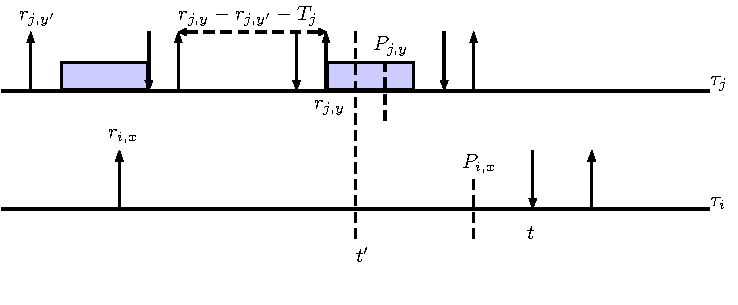
\includegraphics[scale=0.7]{Figure/C1}  
\caption{$ P_{j,y}\leq P_{i,x}$}
  \label{fig:case1}
\end{figure}






\begin{figure}[h!]
 \centering
\includegraphics[scale=0.7]{Figure/C2}  
\caption{$P_{j,y}> P_{i,x}$}
  \label{fig:case2}
\end{figure}

\textbf{Case 2} ($P_{j,y}> P_{i,x}$):~as shown in  Figure~\ref{fig:case2}, $J_{i,x}$ has higher priority than $J_{j,y}$'s  during $[\max(r_{j,y},P_{i,x}),P_{j,y}]$ (if $P_{i,x}\leq P_{j,y}$). Thus  $J_{j,y}$ can not execute  during $[\max(r_{j,y},P_{i,x}),P_{j,y}]$ unless $J_{i,x}$ has already finished. Thus we have
	\begin{align*}
		&f_i(\tau_j,t',t)=\lfloor \frac{t'}{T_j}\rfloor.C_j +
\\&\min\left(C_j,\!t'\!-\!r_{j,y}\!-\!\left[\min(t'\!,\!P_{j,y})\!-\!\max(r_{j,y},\!P_{i,x})\right]_0\right)
		\end{align*}




% 
\subsection{$f_i(\tau_j,t',t)$ when $j> i$}
In this section we consider the case when $\tau_j$ has lower origin priority (higher index) than $\tau_i$. 

\textbf{Case 1.1} ($P_{i,x}\leq P_{j,y}\wedge r_{j,y}\leq r_{i,x}$): as shown in  Figure~\ref{fig:case3}, $\tau_j$ may execute during $[r_{j,y},r_{i,x}]$, but $J_{j,y}$ would not execute after $r_{i,x}$  unless $J_{i,x}$ has finished. Thus we have

	\begin{figure}[h!]
 \centering
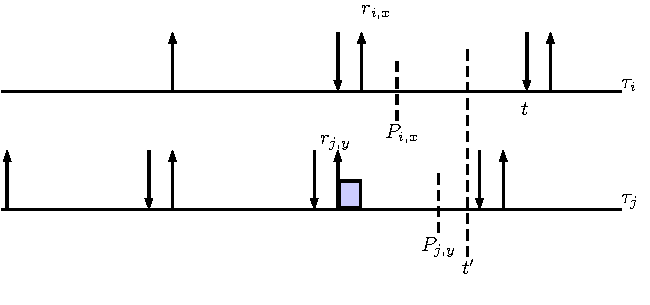
\includegraphics[scale=0.7]{Figure/C3}  
\caption{$P_{i,x}\leq P_{j,t}\wedge r_{j,y}\leq r_{i,x}$}
  \label{fig:case3}
\end{figure}
		\begin{align*}
		f_i(\tau_j,t',t)=\lfloor \frac{t'}{T_j}\rfloor\times C_j+\min(C_j,r_{i,x}-r_{j,y})
	\end{align*}



\textbf{Case 1.2} ($P_{i,x}\leq P_{j,y}\wedge r_{j,y}> r_{i,x}$): as shown in  Figure~\ref{fig:case4},  $J_{j,y}$ would not execute unless $J_{i,x}$ has completed. Thus we have
\begin{align*}
		f_i(\tau_j,t',t)=\lfloor \frac{t'}{T_j}\rfloor\times C_j
\end{align*}

\begin{figure}[h!]
 \centering
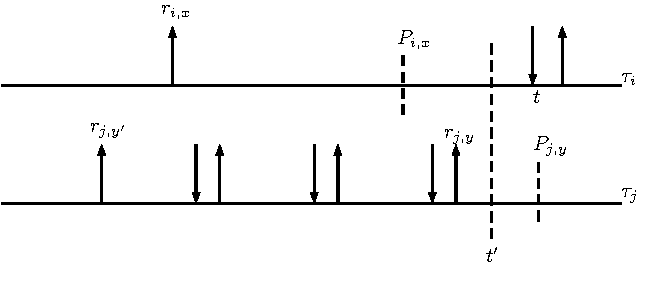
\includegraphics[scale=0.7]{Figure/C31}  
\caption{$P_{i,x}\leq P_{j,y}\wedge r_{j,y}> r_{i,x}$}
  \label{fig:case4}
\end{figure}



\textbf{Case 2.1} ($P_{i,x}>P_{j,y}\wedge r_{j,y}\leq r_{i,x}$): as shown in  Figure~\ref{fig:case5}, after $r_{i,x}$,  $J_{j,y}$ can only execute during $[\max(r_{i,x},P_{j,y}),	\min(t',P_{i,x})]$. Thus we have
	\begin{align*}
		&f_i(\tau_j,t',t)=\lfloor \frac{t'}{T_j}\rfloor\times C_j+\\
		&\min\left(C_j,r_{i,x}-r_{j,y}+[\min(t',P_{i,x})-\max(P_{j,y},r_{i,x})]_0\right)
	\end{align*}


\begin{figure}[h!]
 \centering
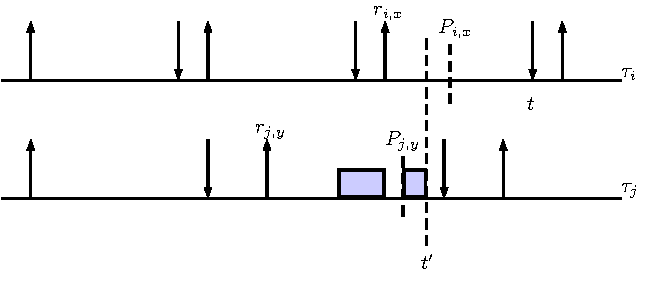
\includegraphics[scale=0.7]{Figure/C4}  
\caption{$P_{i,x}>P_{j,y}\wedge r_{j,y}\leq r_{i,x}$}
  \label{fig:case5}
\end{figure}

\begin{figure}[h!]
 \centering
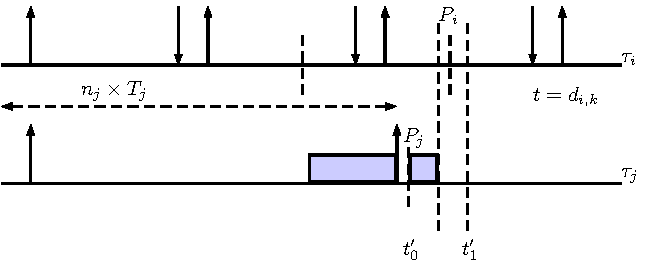
\includegraphics[scale=0.7]{Figure/C41}  
\caption{$P_{i,x}>P_{j,y}\wedge r_{j,y}> r_{i,x} $}
  \label{fig:case6}
\end{figure}

\textbf{Case 2.2} ($P_{i,x}>P_{j,y}\wedge r_{j,y}> r_{i,x}$): as shown in  Figure~\ref{fig:case6}, $J_{j,y}$ would only execute during $[P_{j,y},P_{i,x}]$ before $J_{i,x}$ finishes. Thus we have
\begin{align*}
	f_i(\tau_j,t',t)=&\min\left(C_j,[\min(t',P_{i,x})-P_{j,y}]_0\right)\\&+\lfloor \frac{t'}{T_j}\rfloor\times C_j
\end{align*}







\section{Optimization Technique}
Since the total exectuion happens before $P_{i,x}$ could not exceed $P_{i,x}$, we will introduce an optimization technique based on this fact.  Since  $f_i(\tau_j,t',t)$ denotes the maximum resource used by $\tau_j$ during $[0,t']$, and here we denfine another function $g_i(\tau_j,t')$ which denotes the maximum possible resource used by $\tau_j$ during $[P_{i,x},t']$ (only if $P_{i,x}<t'$).

% \subsection{$g_i(\tau_j,t',t)$  }
\begin{lemma}
If $D_j-p_j\geq C_j$, then $g_i(\tau_j,t')$ maximizes when $r_{j,y'}=[P_{i,x}+C_j-D_j]_0$ and  $r_{j,y}=r_{j,y'}+\lfloor \frac{t'-r_{j,y'}}{T_j}\rfloor T_j$, as shown in Figure~\ref{fig:o1}.
\end{lemma}
\begin{proof}
Case 1: If $P_{i,x}+C_j-D_j\geq 0\Rightarrow r_{j,y'}=P_{i,x}+C_j-D_j$, (scenario in Figure~\ref{fig:o1}) as we shift the pattern left, $J_{j,y'}$ execution after $P_{i,x}$ will decrease linearly up to $C_j$, while  execution of $J_{j,y}$  will increase at most linearly. On the other hand, as we shift the pattern right, $g_i(\tau_j,t')$  would only decrease or stay the same.

Case 2 :If $P_{i,x}+C_j-D_j<0\Rightarrow r_{j,y'}=0$, as we shift the pattern left, execution of $J_{j,y'}$ decreases from $C_j$ to 0, while the increase of $J_{j,y}$ is bounded by $C_j$. On the other hand, as we shift the pattern right, $g_i(\tau_j,t',t)$  would only decrease or stay the same.
\end{proof}

\begin{figure}[h!]
 \centering
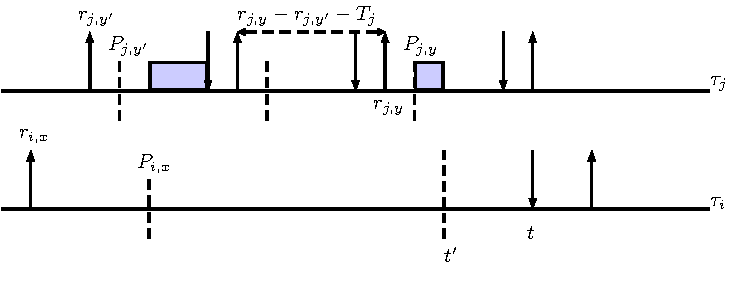
\includegraphics[scale=0.7]{fig/Cx}  
\caption{1}
  \label{fig:o1}
\end{figure}

With the above lemma, we have

	\begin{align}
	\begin{split}
	g_{i}(\tau_j,t',t)=
	\begin{cases}
	&\min(C_j, t'-P_{i,x})~\mbox{~~~~~~~if } r_{j,y}= r_{i,y'}\\
	&C_j+\frac{r_{j,y}-r_{j,y'}-T_j}{T_j}C_j\\&+\min(C_j, [t'-P_{j,y]_0})\mbox{~~~otherwise} \\
	\end{cases}
	\end{split}
	\end{align}

\begin{lemma}
If $D_j-p_j<C_j$, then $g_i(\tau_j,t')$ maximizes when $r_{j,y'}=[P_{i,x}-p_j]_0$ and  $r_{j,y}=r_{j,y'}+\lfloor \frac{t'-r_{j,y'}}{T_j}\rfloor T_j$, as shown in Figure~\ref{fig:o2}.
\end{lemma}
\begin{proof}
Each job of $J_y$ could execute at most $D_j-p_j$ time units after $P_{i,x}$ before $J_{i,x}$ finishes.
Case 1: If $P_{i,x}-p_j\geq 0\Rightarrow r_{j,y'}=P_{i,x}-p_j$ (scenario in Figure~\ref{fig:o1}) as we shift the pattern left, $J_{j,y'}$ execution after $P_{i,x}$ will decrease linearly up to $D_j-p_j$, while  execution of $J_{j,y}$  will increase at most linearly. On the other hand, as we shift the pattern right, $g_i(\tau_j,t',t)$  would only decrease or stay the same.

Case 2 :If $P_{i,x}-p_j<0\Rightarrow r_{j,y'}=0$, as we shift the pattern left, execution of $J_{j,y'}$ decreases from $D_j-p_j$ to 0, while the increase of $J_{j,y}$ is bounded by $D_j-p_j$. On the other hand, as we shift the pattern right, $g_i(\tau_j,t',t)$  would only decrease or stay the same.
\end{proof}


\begin{figure}[h!]
 \centering
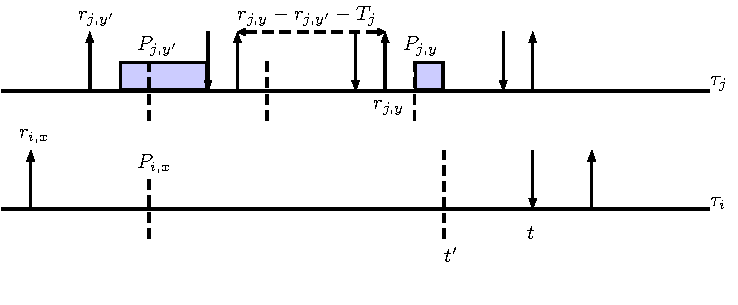
\includegraphics[scale=0.7]{fig/Cy}  
\caption{1}
  \label{fig:o2}
\end{figure}
With the above lemma, we have
	\begin{align*}
	\begin{split}
	g_{i}(\tau_j,t',t)=
	\begin{cases}
	&\min(D_j-p_j, t'-P_{i,x})~\mbox{~~~~~if } r_{j,y}= r_{i,y'}\\
	&D_j-p_j+\frac{r_{j,y}-r_{j,y'}-T_j}{T_j}(D_j-p_j)\\&+\min(D_j-p_j, [t'-P_{j,y]_0})\mbox{~otherwise} \\
	\end{cases}
	\end{split}
	\end{align*}

% \subsection{Optimized test}
Since total execution before $P_{i,x}$ (if $t'>P_{i,x}$) is bounded by  $P_{i,x}$, we can use a simple optimization technique to further tighten the test. 	For $\tau_i$ itself,  its maximum possible execution after  $P_{i,x}$ is $C_j$. Therefore we have 

\begin{equation}
\begin{split}
F_i(\tau,t',t)=~~~~~~~~~~~~~~~~~~~~~~~~~~~~~~~~~~~~~~~~~~~~~~\\
\begin{cases}
& \sum\limits_{\tau_j\in\{\tau\setminus\tau_i\}}f_i(\tau_j,t',t)+ \lfloor \frac{t-D_i}{T_i} \rfloor C_i\mbox{~If~} t'\leq P_{i,x}\\
&\min\!\left(P_{i,x},  \lfloor \frac{t-D_i}{T_i} \rfloor C_i\!\!+\!\!\!\!\!\!\!\sum\limits_{\tau_j\in\{\tau\setminus\tau_i\}}\!\!\!\!\!\!f_i(\tau_j,t',t)\!-\!g_{i}(\tau_j,t',t)\!\right)\\&+\sum_{\tau_j\in\{\tau\setminus\tau_i\}}g_{i}(\tau_j,t',t)\mbox{~~~~~~~~~~~~~Otherwise}
\end{cases}	
\end{split}
\end{equation}





 

We also need to derive an upper bound of $t$ because otherwise $t$ can tends to infinity. Suppose there exists a $t$ so that
\begin{align*}
\forall~t'\in(t-D_i,t]:~F_i(\tau,t,t')+C_i>t'\\
\Rightarrow\min_{t'\in(t-D_i,t]}\frac{F(\tau_i,t,t')+C_i}{t'}>1	
\end{align*}

, and let
\begin{align*}
H_i(t)= & U\times t+\sum_{\tau_j\in\{\tau\setminus\tau_i\}}C_j+C_i\\&\geq t\times u_i+\sum_{\tau_j\in\{\tau\setminus\tau_i\}}(\lfloor \frac{t'}{T_j} \rfloor+1)C_j+C_i\\
&\geq F(\tau_i,t,t')+C_i
\end{align*}
Then it must be that

\begin{align*}
&\frac{H_i(t)}{t-D_i}>1\Rightarrow t-D_i< U\times t+\sum_{\tau_j\in\{\tau\}}C_j\\
&\Rightarrow t<\frac{D_i+\sum_{\tau_j\in\tau}C_j}{1-U}
\end{align*}

% \section{Draft Simulation Results}

% \begin{table}[h]
% \caption{Notations}
% \label{tab:x}
% \large
% \center
% \begin{tabular}{|l|l|l|l|l|}
%  \hline
% Uniform Distribution&[0.88,0.9]&[0.93,0.95]&[0.95,0.97]&[0.97,0.99]\\
%  \hline
% Acceptance Ratio&1&1&0.995&0.982\\
%  \hline
% \end{tabular}
% \end{table}




% \begin{equation}
% \begin{split}
% rbf_i(\tau-\tau_i,t')=
% \begin{cases}
% &\min\{r_{i,x}, \sum_{\tau_j\in \tau-\tau_i}rbf_i(\tau_j,t')-rbf_i^1(\tau_j,t') \}\\&+\sum_{\tau_j\in \tau-\tau_i}rbf_i^1(\tau_j,t') 								\mbox{if } t'<=P_i\\
% 				fa						&\mbox{otherwise}
% \end{cases}	
% \end{split}
% \end{equation}












\end{document}  